%! Author = vova
%! Date = 26.09.2020

% Preamble
\documentclass[11pt]{article}

% Packages
\usepackage{amsmath}
\usepackage{romannum}
\usepackage{hyperref}
\usepackage{graphicx}

\title{On non-ideal voltage and current measurement tools}
\date{26.09.2020}
\author{Latipov Vladimir \&\& Onishenko Sergiy}


% Document
\begin{document}
    \pagenumbering{gobble}
    \maketitle
    \newpage
    \pagenumbering{arabic}

    \section{Abstract}\label{sec:abstract}
    It`s contents should be too abstract for me to be able to write it.

    \section{Experiments}\label{sec:experiments}
    There were 4 experiments arranged:

        \subsection{Experiment \textnumero1: Sequential plugging in}\label{subsec:experiment-1} % \Romannum{1}
    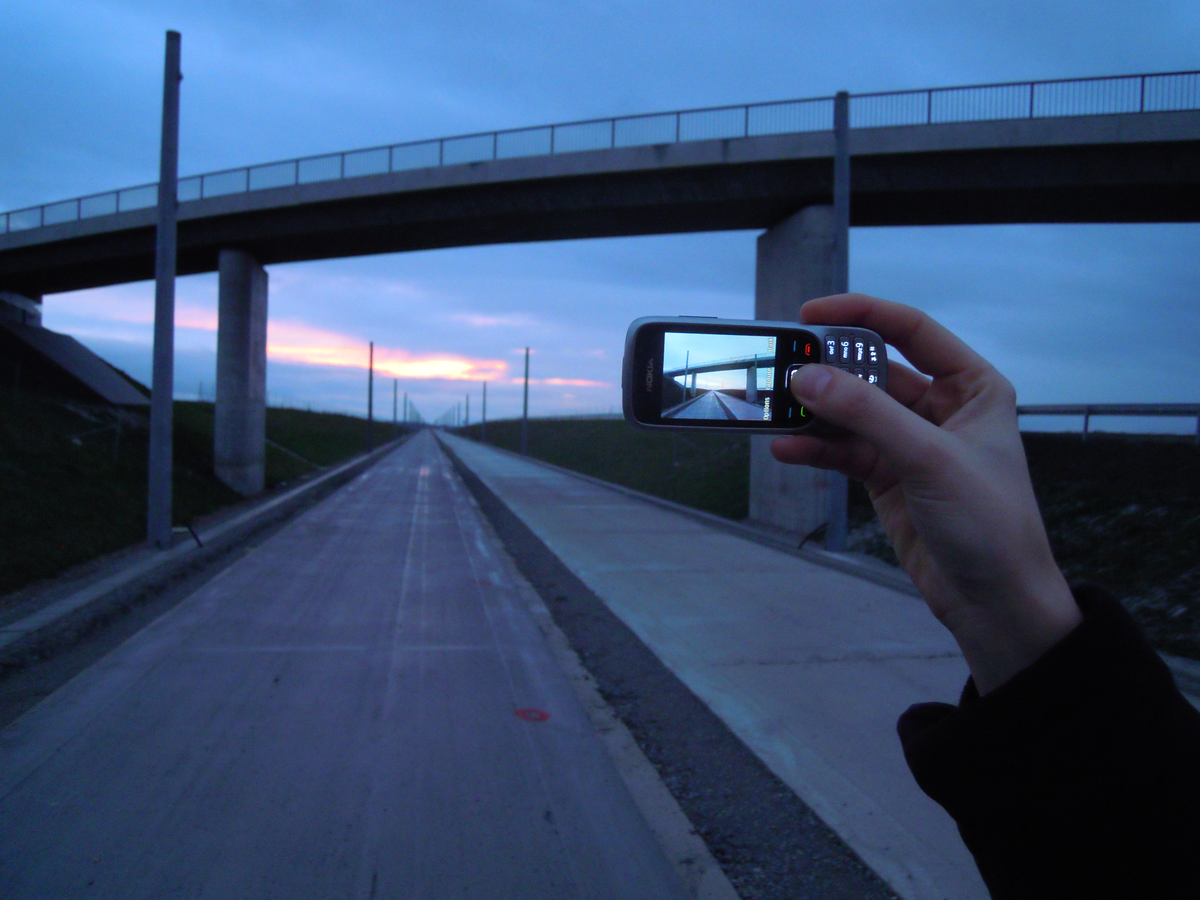
\includegraphics[width=\linewidth]{images/schemes/scheme0.png}

    \subsection{Experiment \textnumero2: Only Voltmeter}\label{subsec:experiment-2}
    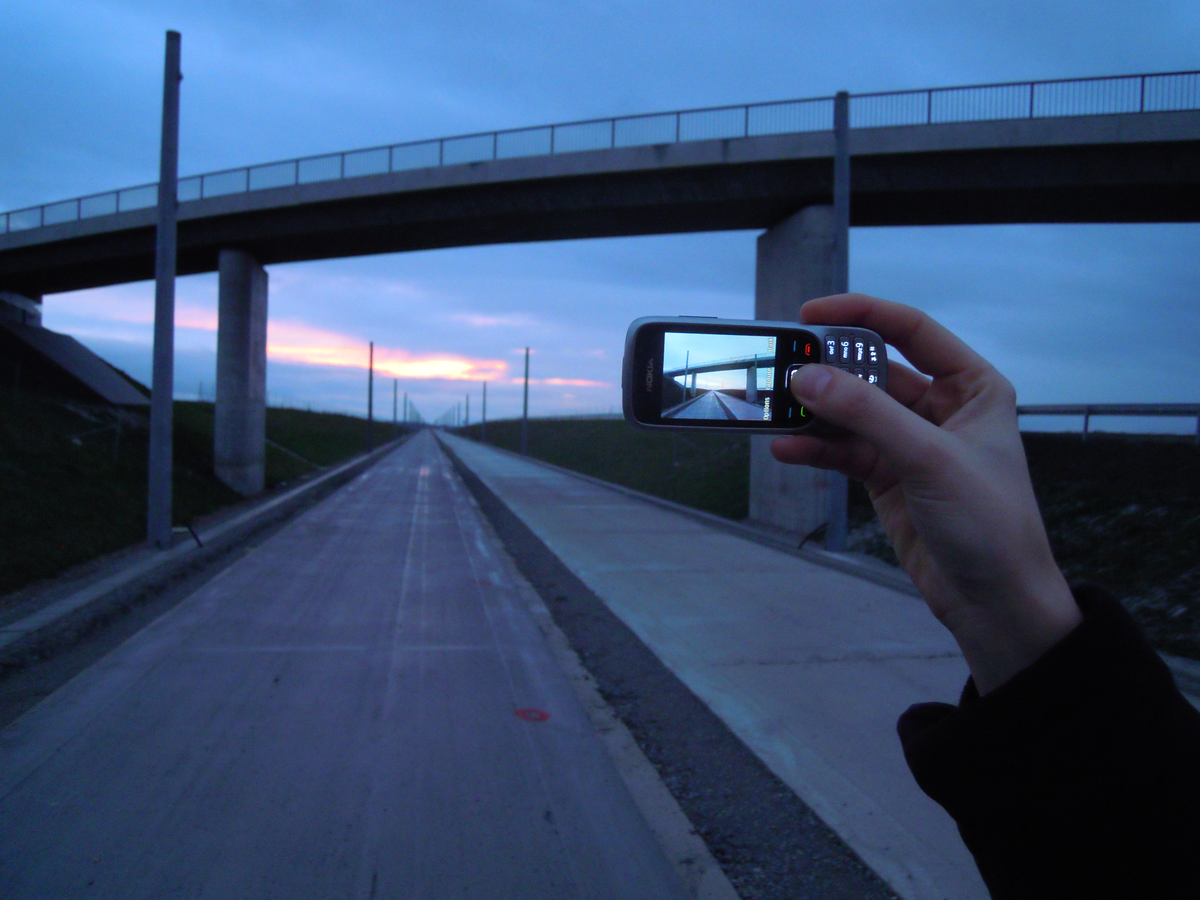
\includegraphics[width=\linewidth]{images/schemes/scheme0.png}

    \subsection{Experiment \textnumero3: Only Ampermeter}\label{subsec:experiment-3}
    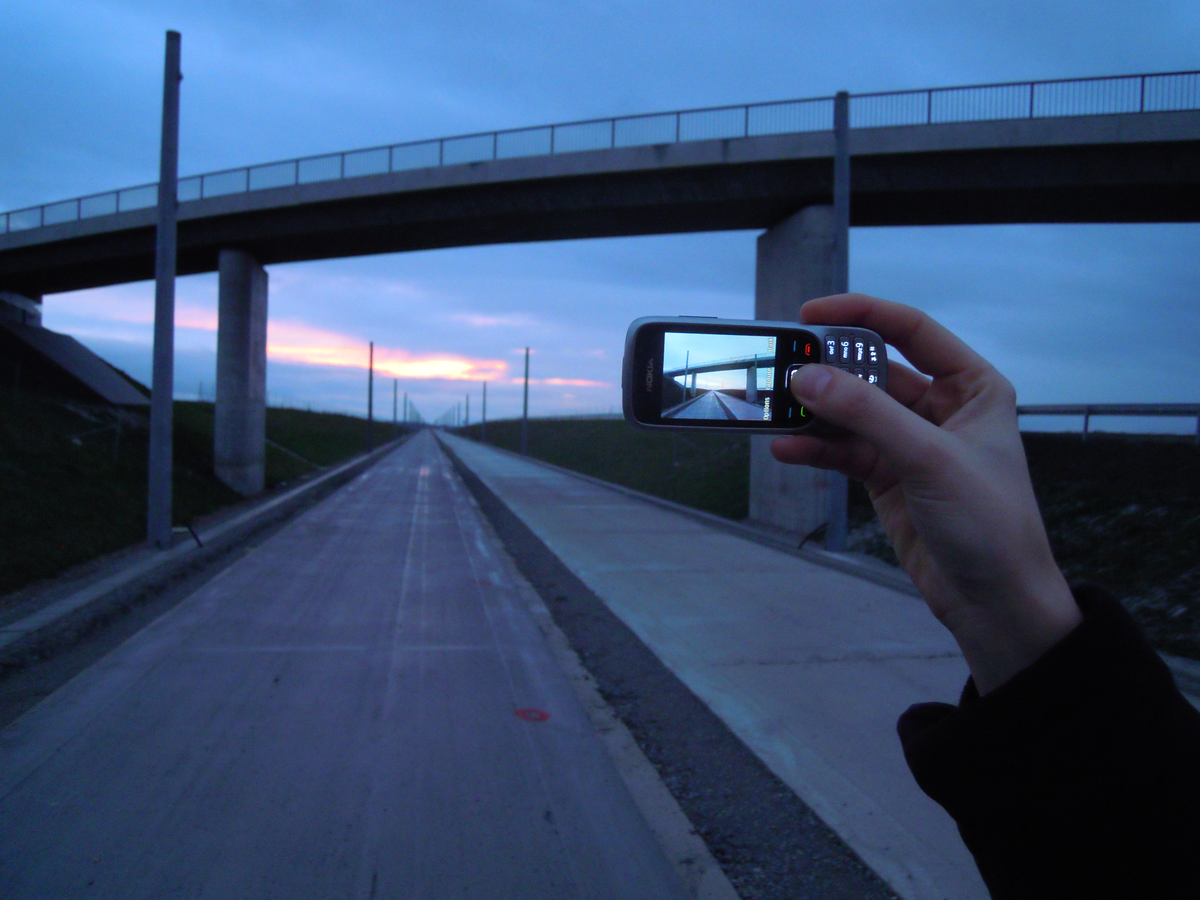
\includegraphics[width=\linewidth]{images/schemes/scheme0.png}


    \section{Solving equation system}\label{sec:solving-equation-system}

    \begin{equation}
        A_1 = \frac{\varepsilon}{I}\label{eq:equation2}
    \end{equation}

    \begin{equation}
        V_1 = \frac{\varepsilon \cdot R_v}{I}\label{eq:equation}
    \end{equation}

    \begin{equation*}
        R_v = \frac{V_1}{A_1}
    \end{equation*}

    \begin{equation}
        V_2 = \varepsilon \cdot \frac{R_v}{R_v + R_\varepsilon}\label{eq:equation3}
    \end{equation}

    \begin{equation*}
        \varepsilon = V_2 + V_2 \cdot \frac{R_\varepsilon}{R_v}
    \end{equation*}

    \begin{equation}
        A_3 = \varepsilon \cdot \frac{1}{R_A + R_\varepsilon} = (V_2 + V_2 \cdot \frac{R_\varepsilon}{R_v}) \cdot \frac{1}{R_A + R_\varepsilon} \label{eq:equation4}
    \end{equation}




\end{document}